\documentclass[11pt,letterpaper]{article}
\usepackage[lmargin=1in,rmargin=1in,tmargin=1in,bmargin=1in]{geometry}
\usepackage{../style/homework}
\usepackage{../style/commands}
\setbool{quotetype}{true} % True: Side; False: Under
\setbool{hideans}{true} % Student: True; Instructor: False

% -------------------
% Content
% -------------------
\begin{document}

\homework{10: Due 10/30}{The study of mathematics, like the Nile, begins in minuteness but ends in magnificence.}{Charles Caleb Colton}

% Problem 1
\problem{10} Consider the relation $f$ plotted below. 
	\[
	\fbox{
	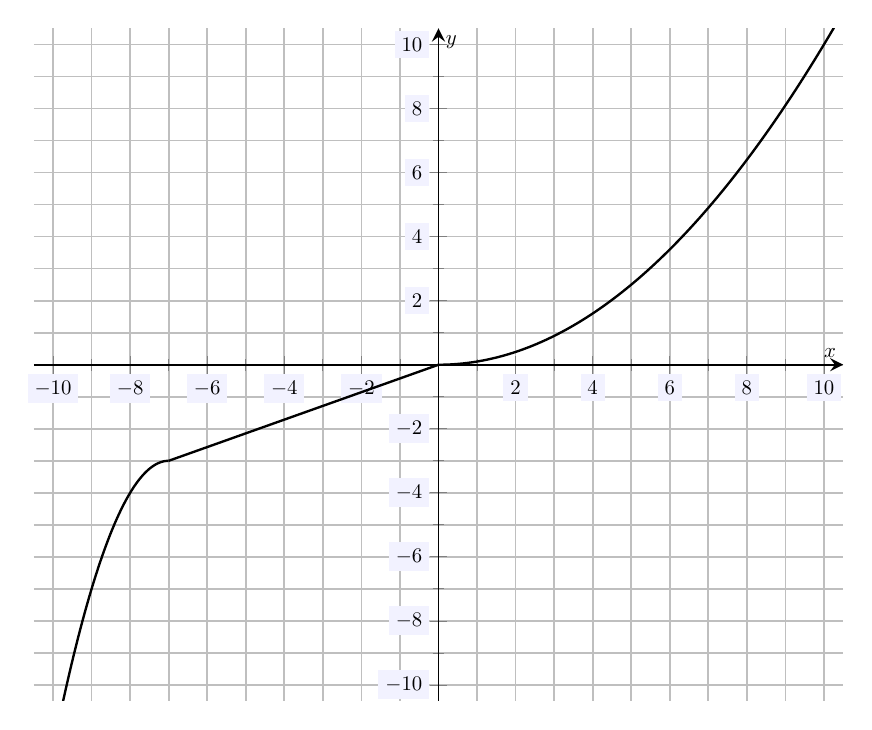
\begin{tikzpicture}[scale=1.5,every node/.style={scale=0.5}]
	\begin{axis}[
	grid=both,
	axis lines=middle,
	ticklabel style={fill=blue!5!white},
	xmin= -10.5, xmax=10.5,
	ymin= -10.5, ymax=10.5,
	xtick={-10,-8,-6,-4,-2,0,2,4,6,8,10},
	ytick={-10,-8,-6,-4,-2,0,2,4,6,8,10},
	minor tick = {-10,-9,...,10},
	xlabel=\(x\),ylabel=\(y\),
	]
	\addplot[line width= 0.02cm,samples=100,domain= -10.5:-7] ({x},{-(x + 7)^2 - 3}); 
	\addplot[line width= 0.02cm,samples=100,domain= -7:0] ({x},{3/7*x}); 
	\addplot[line width= 0.02cm,samples=100,domain= 0:10.5] ({x},{x^2/10}); 
	\end{axis}
	\end{tikzpicture}
	}
	\] 

\begin{enumerate}[(a)]
\item Compute $f(7)$ and $f(-9)$. 
\item Is $f(x)$ a function? Explain. 
\item Does $f(x)$ have an inverse? If so, sketch the inverse. If not, explain why. 
\end{enumerate}



\newpage



% Problem 2
\problem{10} Showing all your work, verify that $g(x)= 4x + 9$ is the inverse function for $f(x)= \frac{x - 9}{4}$. Also, compute $g(-2)$. What does the value of $g(-2)$ tell you about the function $f(x)$? 



\newpage



% Problem 3
\problem{10} A relation $\phi$ is plotted below. 
	\[
	\fbox{
	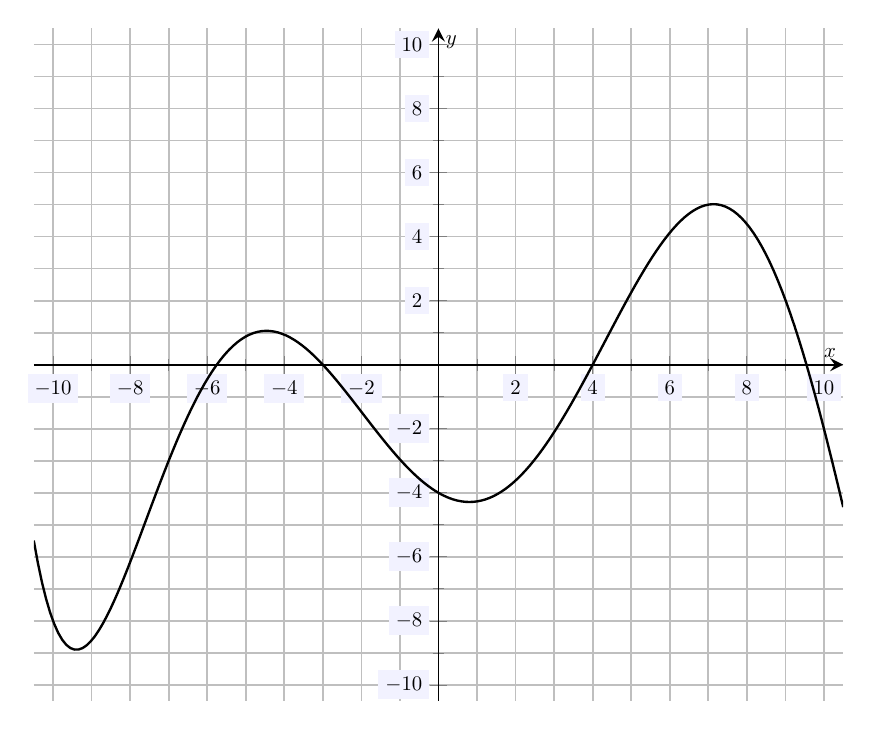
\begin{tikzpicture}[scale=1.5,every node/.style={scale=0.5}]
	\begin{axis}[
	grid=both,
	axis lines=middle,
	ticklabel style={fill=blue!5!white},
	xmin= -10.5, xmax=10.5,
	ymin= -10.5, ymax=10.5,
	xtick={-10,-8,-6,-4,-2,0,2,4,6,8,10},
	ytick={-10,-8,-6,-4,-2,0,2,4,6,8,10},
	minor tick = {-10,-9,...,10},
	xlabel=\(x\),ylabel=\(y\),
	]
	\addplot[line width= 0.02cm,samples=200,domain= -10.5:10.5] ({x},{-4. - 0.695759*x + 0.394934*x^2 + 0.0411407*x^3 - 0.00782987*x^4 - 0.000311831*x^5 + 0.0000378053*x^6}); 
	\end{axis}
	\end{tikzpicture}
	}
	\] 
Using the plot above, answer the following:
	\begin{enumerate}[(a)]
	\item Compute $\phi(9)$.
	\item Find the $y$-intercept for $\phi(x)$. 
	\item Find the $x$-intercepts for $\phi(x)$. 	
	\item As accurately as possible, compute the preimage of $-3$, i.e. $\phi^{-1}(-3)$. 
	\item Explain why (d) implies that $\phi$ does not have an inverse function. 
	\end{enumerate}


\end{document}